\section{Realworld Bimanual Tasks}
\label{sec:eval_bimanual}
Beyond single arm setup, we further demonstrate Diffusion Policy on several challenging bimanual tasks. To enable bimanual tasks, the majority of effort was spent on extending our robot stack to support multi-arm teleopration and control. Diffusion Policy worked out of the box for these tasks without hyperparameter tuning. 

\subsection{Observation and Action Spaces}
The proprioceptive observation space is extended to include the poses of both end-effectors and the gripper widths of both grippers. We also extend the observation space to include the actual and desired values of these quantities.
The image observation space is comprised of two scene cameras and two wrist cameras, one attached to each arm.
The action space is extended to include the desired poses of both end-effectors and the desired gripper widths of both grippers.

\subsection{Teleoperation}
For these coordinated bimanual tasks, we found using 2 SpaceMouse simultaneously quite challenging for the demonstrator. Thus, we implemented two new teleoperation modes:
using a Meta Quest Pro VR device with two hand controllers, or
haptic-enabled control using 2
\href{https://www.haption.com/en/products-en/virtuose-6d-tao-en.html\#fa-download-downloads}{
Haption Virtuose\legalTM\ 6D HF TAO}
devices using bilateral position-position coupling as described succinctly in the haptics section of \citet{siciliano2008springer}. This coupling is performed between a Haption device and a Franka Panda arm.
More details on the controllers themselves may be found in Sec. \ref{sec:franka_setup}.
The following provides more details on each task and policy performance.  

\subsection{Bimanual Egg Beater}

The bimanual egg beater task is illustrated and described in Fig. \ref{fig:real_egg_beater}, using a
\href{https://www.oxo.com/egg-beater.html}{OXO\legalTM Egg Beater} and a
\href{https://www.target.com/p/114oz-plastic-serving-bowl-jet-gray-room-essentials-8482/-/A-86701588}{Room Essentials\legalTM plastic bowl}. We chose this task to illustrate the importance of haptic feedback for teleoperating bimanual manipulation even for common daily life tasks such as coordinated tool use. Without haptic feedback, an expert was unable to successfully complete a single demonstration out of 10 trials. 5 failed due to robot pulling the crank handle off the egg beater; 3 failed due to robot losing grasp of the handle; 2 failed due to robot triggering torque limit. In contrast, the same operator could easily perform this task 10 out of 10 times with haptic feedback. Using haptic feedback made it possible for the demonstrations to be both quicker and higher quality than without feedback.

\begin{figure}[t]
\centering
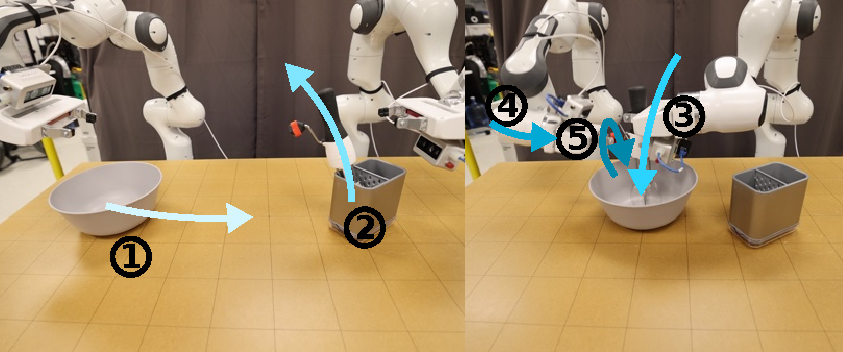
\includegraphics[width=\linewidth]{figure/real_egg_beater_setup_compressed.pdf}
\caption{\textbf{Bimanual Egg Beater Manipulation. } 
\label{fig:real_egg_beater}
The robot needs to
\textcircled{\raisebox{-0.9pt}{1}} push the bowl into position (only if too close to the left arm),
\textcircled{\raisebox{-0.9pt}{2}} approach and pick up the egg beater with the right arm,
\textcircled{\raisebox{-0.9pt}{3}} place the egg beater in the bowl,
\textcircled{\raisebox{-0.9pt}{4}} approach and grasp the egg beater crank handle, and
\textcircled{\raisebox{-0.9pt}{5}} turn the crank handle 3 or more times.
}
\vspace{-4mm}
\end{figure}

\textbf{Result Analysis.} Diffusion policy is able to complete this task with 55\% success rate over 20 trials, trained using 210 demonstrations. The primary failure modes for these were out-of-domain initial positioning of the egg beater, or missing the egg beater crank handle or losing grasp of it. The initial and final states for all rollouts are visualized in \ref{fig:egg_beater_ini} and \ref{fig:egg_beater_last}.



\subsection{Bimanual Mat Unrolling}

The mat unrolling task is shown and described in Fig. \ref{fig:real_unroll_mat}, using a
\href{https://www.amazon.com/DogBuddy-Dog-Food-Mat-Waterproof/dp/B08GGDNB71}{XXL Dog Buddy\legalTM Dog Mat}.
This task was teleoperated using the VR setup, as it did not require rich haptic feedback to perform the task. We taught this skill to be omnidextrous, meaning it can unroll either to the left or right depending on the initial condition.

\begin{figure}[t]
\centering
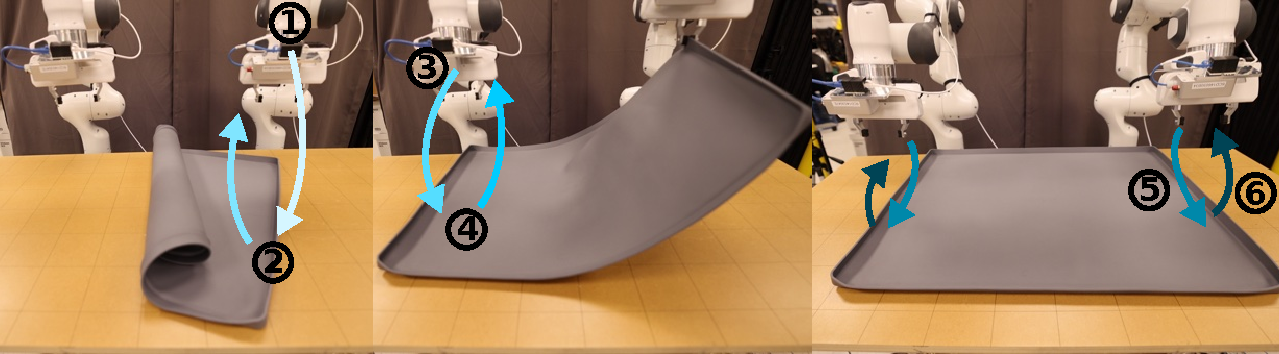
\includegraphics[width=\linewidth]{figure/real_unroll_mat_setup_compressed.pdf}
\caption{\textbf{Bimanual Mat Unrolling. } 
\label{fig:real_unroll_mat}
The robot needs to
\textcircled{\raisebox{-0.9pt}{1}} pick up one side of the mat (if needed), using the left or right arm,
\textcircled{\raisebox{-0.9pt}{2}} lift and unroll the mat (if needed),
\textcircled{\raisebox{-0.9pt}{3}} ensure that both sides of the mat are grasped,
\textcircled{\raisebox{-0.9pt}{4}} lift the mat,
\textcircled{\raisebox{-0.9pt}{5}} place the mat oriented with the table, mostly centered, and
\textcircled{\raisebox{-0.9pt}{6}} release the mat.
}
\vspace{-4mm}
\end{figure}

\textbf{Result Analysis.} Diffusion policy is able to complete this task with 75\% success rate over 20 trials, trained using 162 demonstrations. The primary failure modes for these were missed grasps during initial grasp of the mat, where the policy struggled to correct itself and thus got stuck repeating the same behavior. The initial and final states for all rollouts are visualized in \ref{fig:unroll_mat_ini} and \ref{fig:unroll_mat_last}.

\subsection{Bimanual Shirt Folding.}
The shirt folding task is described and illustrated in Fig. \ref{fig:real_fold_shirt}, using a short-sleeve T-shirt. This task was also teleoperated using the VR setup as it did not require rich
feedback to perform the task. Due to the kinematic and workspace constraints, this task is notably longer and can take up to nine discrete steps. The last few steps require both grippers to come very close towards each other. Having our mid-level controller explicitly handling collision avoidance was especially important for both teleoperation and policy rollout. 

\begin{figure}[t]
\centering
% TODO(eric): Couldn't get the PDF to fit under 50 MB
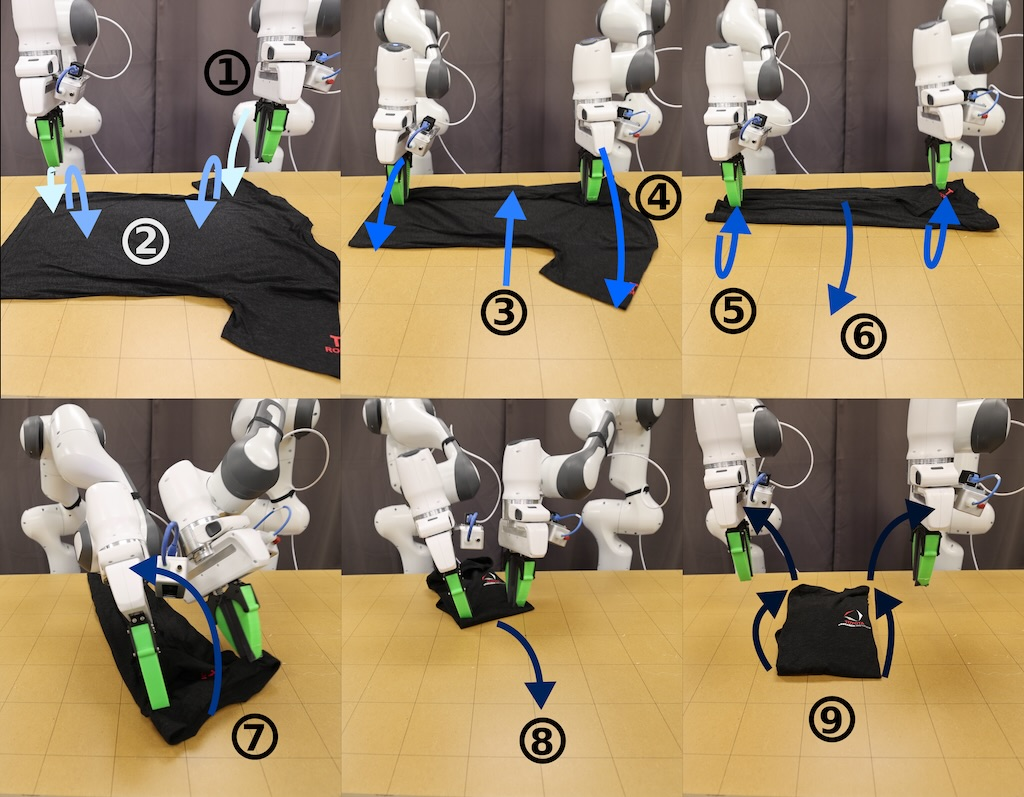
\includegraphics[width=\linewidth]{figure/real_fold_shirt_setup.jpg}
\caption{\textbf{Bimanual Shirt Folding. } 
\label{fig:real_fold_shirt}
The robot needs to
\textcircled{\raisebox{-0.9pt}{1}} approach and grasp the closest sleeve with both arms,
\textcircled{\raisebox{-0.9pt}{2}} fold the sleeve and release,
\textcircled{\raisebox{-0.9pt}{3}} drag the shirt closer (if needed),
\textcircled{\raisebox{-0.9pt}{4}} approach and grasp the other sleeve with both arms,
\textcircled{\raisebox{-0.9pt}{5}} fold the sleeve and release,
\textcircled{\raisebox{-0.9pt}{6}} drag the shirt to a orientation for folding,
\textcircled{\raisebox{-0.9pt}{7}} grasp and fold the shirt in half by its collar,
\textcircled{\raisebox{-0.9pt}{8}} drag the shirt to the center, and
\textcircled{\raisebox{-0.9pt}{9}} smooth out the shirt and move the arms away.
}
\vspace{-4mm}
\end{figure}

\textbf{Result Analysis.} Diffusion policy is able to complete this task with 75\% success rate over 20 trials, trained using 284 demonstrations. The primary failure modes for these were missed grasps for initial folding (the sleeves and the color), and the policy being unable to stop adjusting the shirt at the end. The initial and final states for all rollouts are visualized in \ref{fig:fold_shirt_ini} and \ref{fig:fold_shirt_last}.



